\documentclass[tikz,border=3pt]{standalone}
\usepackage[T1]{fontenc}
\usepackage{amsmath}
\usepackage{XCharter}
\usepackage[xcharter]{newtxmath}
\usepackage[scaled=.92]{helvet}
\usepackage{pgfplots}
\usetikzlibrary{arrows.meta,positioning,fit,calc,backgrounds,decorations.pathreplacing,patterns}
\usepgfplotslibrary{groupplots,fillbetween}
\pgfplotsset{compat=1.18}
\definecolor{ink}{HTML}{172536}
\definecolor{rgb}{HTML}{3563B8}
\definecolor{event}{HTML}{17857C}
\definecolor{fusion}{HTML}{76529C}
\definecolor{reference}{HTML}{8994A3}
\definecolor{warn}{HTML}{AC5948}
\definecolor{muted}{HTML}{657183}
\definecolor{rule}{HTML}{D9E0E8}
\definecolor{pale}{HTML}{F5F7FA}
\color{ink}
\tikzset{box/.style={rounded corners=2pt,draw=rule,fill=white,align=center,inner sep=4pt,font=\sffamily\fontsize{9}{10.8}\selectfont,minimum height=9mm},rb/.style={box,draw=rgb!50,fill=rgb!5},eb/.style={box,draw=event!50,fill=event!5},fb/.style={box,draw=fusion!55,fill=fusion!5},arrow/.style={-{Latex[length=1.8mm]},line width=.65pt,draw=muted},note/.style={font=\sffamily\fontsize{8.4}{10.2}\selectfont,align=center,text=muted},heading/.style={font=\sffamily\fontsize{10}{12}\selectfont\bfseries,align=left,text=ink}}
\pgfplotsset{paper/.style={width=15.7cm,height=6cm,axis lines*=left,axis line style={rule},tick style={draw=none},tick label style={font=\sffamily\fontsize{8.8}{10.4}\selectfont,text=muted},label style={font=\sffamily\fontsize{9.4}{11}\selectfont,text=ink},title style={font=\sffamily\fontsize{10}{12}\selectfont\bfseries,text=ink},legend style={draw=none,fill=none,font=\sffamily\fontsize{9}{11}\selectfont,cells={anchor=west}},grid=major,grid style={rule!65,line width=.3pt},minor tick num=0,scaled ticks=false,unbounded coords=jump,clip mode=individual}}
\begin{document}

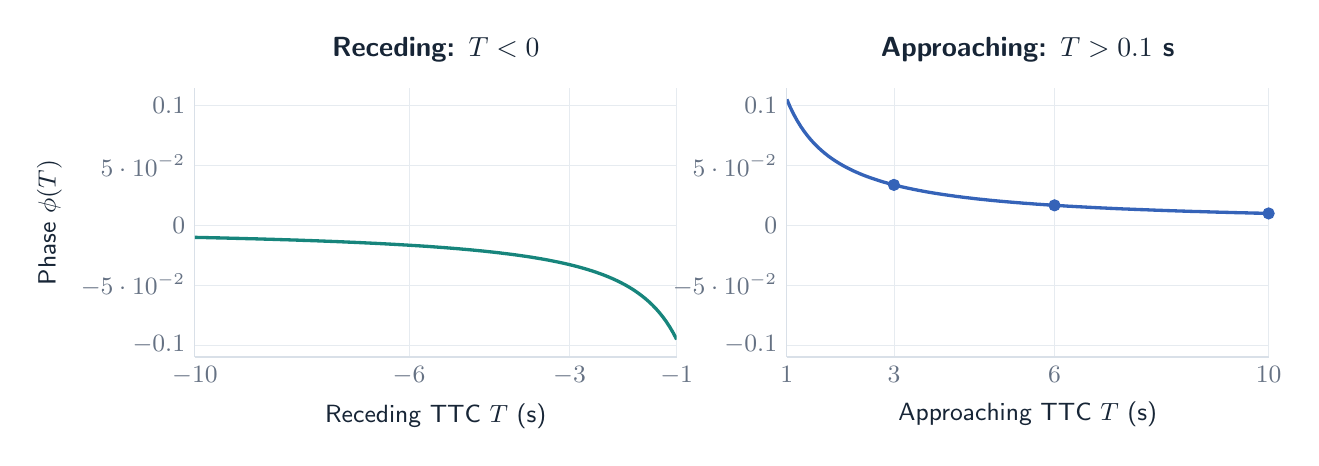
\begin{tikzpicture}
\begin{groupplot}[paper,group style={group size=2 by 1,horizontal sep=1.4cm},width=7.7cm,height=5cm,ylabel={Phase \(\phi(T)\)},ytick={-.1,-.05,0,.05,.1},ymin=-.11,ymax=.115]
\nextgroupplot[xmin=-10,xmax=-1,xtick={-10,-6,-3,-1},xlabel={Receding TTC \(T\) (s)},title={Receding: \(T<0\)}]
\addplot[event,very thick,domain=-10:-1,samples=140] {-ln(1-.1/x)};
\nextgroupplot[xmin=1,xmax=10,xtick={1,3,6,10},xlabel={Approaching TTC \(T\) (s)},ylabel={},title={Approaching: \(T>0.1\) s}]
\addplot[rgb,very thick,domain=1:10,samples=140] {-ln(1-.1/x)};
\addplot[only marks,mark=*,rgb] coordinates {(3,.03390155) (6,.01680712) (10,.01005034)};
\end{groupplot}
\end{tikzpicture}
\end{document}
